\documentclass[11pt,letterpaper,boxed]{hmcpset}
\usepackage{fullpage}
\setlength{\parskip}{6pt}
\setlength{\parindent}{0pt}
\usepackage[margin=1in]{geometry}
\usepackage{graphicx}
\usepackage{enumerate}
\usepackage{marvosym}
\usepackage{amssymb}
\usepackage{wasysym}
\usepackage{gensymb}
\usepackage{mathrsfs}
\usepackage{scrextend}
\usepackage{mathtools}
\usepackage{pgfplots}
\usepackage{xspace}
\usepackage{esvect}
\usepackage{lipsum}
\usepackage{float}
\usepackage{esint}


\name{Name $\rule{4cm}{0.15mm}$}
\class{Physics 51M Section $\rule{.5cm}{0.15mm}$ Box \# $\rule{1cm}{0.15mm}$}
\assignment{Problem Set 7}
\duedate{4 November 2019}

\begin{document}
	
	%\begin{center}
	\noindent\textbf{Collaborators:} 
	%\end{center} 
	
	%\problemlist{}
	
	\begin{problem} (a) Calculate the capacitance per unit length $\frac{C}{L}$ of a cylindrical capacitor (two concentric conducting cylindrical shells, inner radius $a$ and outer radius b) as shown in the figure. Ignore the end-caps of the cylinders.
(b) Commercial RG-58 “BNC” coaxial cable (same geometry as
part (a) above) has an inner cylinder diameter of $0.8 mm$, and an outer diameter of $5 mm$. Calculate the capacitance per unit length
of RG-58 cable, and compare it to the commonly quoted value of 33 $pF/foot$. Comment on your result.
		\begin{center}
		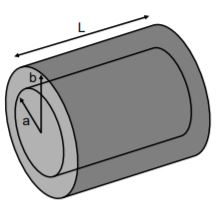
\includegraphics[scale=.7]{51m7pic.jpg}
		\end{center}
		
	\end{problem}
	
	\begin{solution}
		\vfill
	\end{solution}
	\newpage

	\begin{problem}The current density across a cylindrical conductor of radius $R$ 
	varies according to the equation $j = j_0(1 - \frac{r}{R})$, where $r$ is the distance from the axis. Thus the current density is a maximum $j_0$ at the axis $r = 0$
 and decreases linearly to zero at the surface $r = R$.
(a) Calculate the current in terms of $j_0$ and the conductor’s cross-sectional area $A = \pi R^2$.
(b) Suppose that, instead, the current density is a maximum $j_0$ at the surface and decreases linearly to zero at the axis, so that $j = j_0 \frac{r}{R}$. Calculate the current. Why is the answer different from part (a)?

	\end{problem}
	\begin{solution}
		\vfill
	\end{solution}
	\newpage

	\begin{problem}* A dielectric slab of thickness $b$ is inserted between the plates of a parallel-plate capacitor of plate separation $d$. Show that the capacitance is given by $C = \frac{K_e \epsilon_0 A}{k_e d -b(k_e -1)}$.
		
	\end{problem}
	
	\begin{solution}
		\vfill
	\end{solution}
	\newpage	
	
	\begin{problem}[HRK 31.48] A capacitor (capacitance $C$) with an initial stored energy $U_0$ is discharged
through a resistor of resistance $R$. (In parts (a) and (b) below, calculate a final numerical value
assuming $C =1.0 \mu F, U_0 = 0.50 J$, and $R=1 M\Omega$.)\\
(a) What is the initial charge on the capacitor?
(b) What is the current through the resistor when the discharge starts?
(c) Determine $\bigtriangleup VC$, the voltage across the capacitor, and $\bigtriangleup VR$, the voltage across the resistor, as
functions of time.
(d) Express the rate of generation of internal energy in the resistor as a function of time.
	\end{problem}
	
	\begin{solution}
		\vfill
	\end{solution}
	\newpage
	
	\begin{problem}[HRK E32.32]
A metal wire of mass $m$ slides without friction on two horizontal rails spaced a distance $d$ apart, as in Fig 32-36. The track lies in a vertical uniform magnetic field $\vec{B}$. A constant current $i$ flows from generator G along one rail, across the wire, and back down the other rail. Find the velocity (speed and direction) of the wire a s a function of time, assuming it to be at rest at $t = 0$.
\begin{center}
			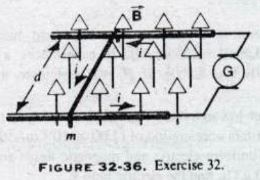
\includegraphics[scale=.7]{51m7pic2.jpg}
	\end{center}
		
	\end{problem}
	
	\begin{solution}
		\vfill
	\end{solution}
	\newpage
	
	\begin{problem}[HRK P32.5] Bainbridge's mass spectrometer, as shown in Fig. 32-39, separates ions having the same velocity. The ions, after entering through slits $S_1$ and $S_2$, pass through a velocity selector composed of an electric field produced by the charged plates $P$ and $P'$, and a magnetic field $\vec{B}$ perpendicular to the electric field and the ion path. Those ions that pass undeviated through the crossed $\vec{E}$ and $\vec{B}$ fields enter into a region where a second magnetic field $\vec{B'}$ exists, and are bent into circular paths. A photographic plate registers their arrival. Show that $\frac{q}{m} = \frac{E}{rBB'}$, where $r$ is the radius of the circular orbit.
\begin{center}
			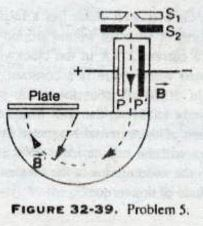
\includegraphics[scale=.7]{51m7pic3.jpg}
	\end{center}
	\end{problem}
	
	\begin{solution}
		\vfill
	\end{solution}
	\newpage
	
	
\end{document}